% !TEX root = ../../main.tex

\subsubsection{MIL-127(Fe)}

The isotherms on the original powder form of MIL-127(Fe)
should show similar behaviour as on MIL-100(Fe),
due to the presence of the same iron trimesate moieties,
although with a sharper uptake as a result of the smaller pores. Enthalpy
profiles are also influenced by the similar interactions with the iron
CUS leading to higher initial heats of adsorption on \ce{CO} and \ce{C3H6}.
An overall increase in the heat of adsorption at higher loadings is seen
throughout the probe series, as seen for example on butane in
\autoref{shaping:fgr:mil127c4h10ads}.
Due to the bimodal pore distribution in the MIL-127(Fe) structure,
it is likely that adsorption first commences in the small
(\( \sim \)\SI{6}{\angstrom}) channels and then, at higher pressures,
intrusion into the larger cage-type pores is possible through the
\( \sim \)\SI{3}{\angstrom} narrow apertures.
The confined cages have an increased interaction with the molecule
which leads to the higher enthalpy values.

When comparing the powder and the pellet variant with respect to
initial Henry's constant, a large difference in \(K_H\) on \ce{CO}
stands out. The value of the initial enthalpy of adsorption
does not follow the same pattern.
However, visual inspection of the enthalpy curve in
\autoref{shaping:fgr:mil127coads} shows that the energy of
adsorption corresponding to
interactions with the more active sites is maintained for a larger
percentage of the total coverage.
This points to the higher preponderence of such sites in the powder
variant. A similar offset can be seen in the propylene enthalpy at very
low pressures, but this is not reflected in the shape of the isotherm.
The weaker complexation strength and the larger size of the molecule
likely limits the effect seen in the carbon monoxide isotherm.
As for the underlying reason behind the isotherm divergence, it
could be that the alumina binder acts as protection against the
generation of iron (II) during thermal activation.
No other differences are seen between the two forms on either Henry
constant and initial enthalpy of adsorption.

\begin{figure}[p!]
	\centering
	\begin{subfigure}{\linewidth}
		\parbox[c]{0.1\linewidth}{\caption{}%
			\label{shaping:fgr:analysismil127henry}}%
		\parbox[b]{0.8\linewidth}{%
			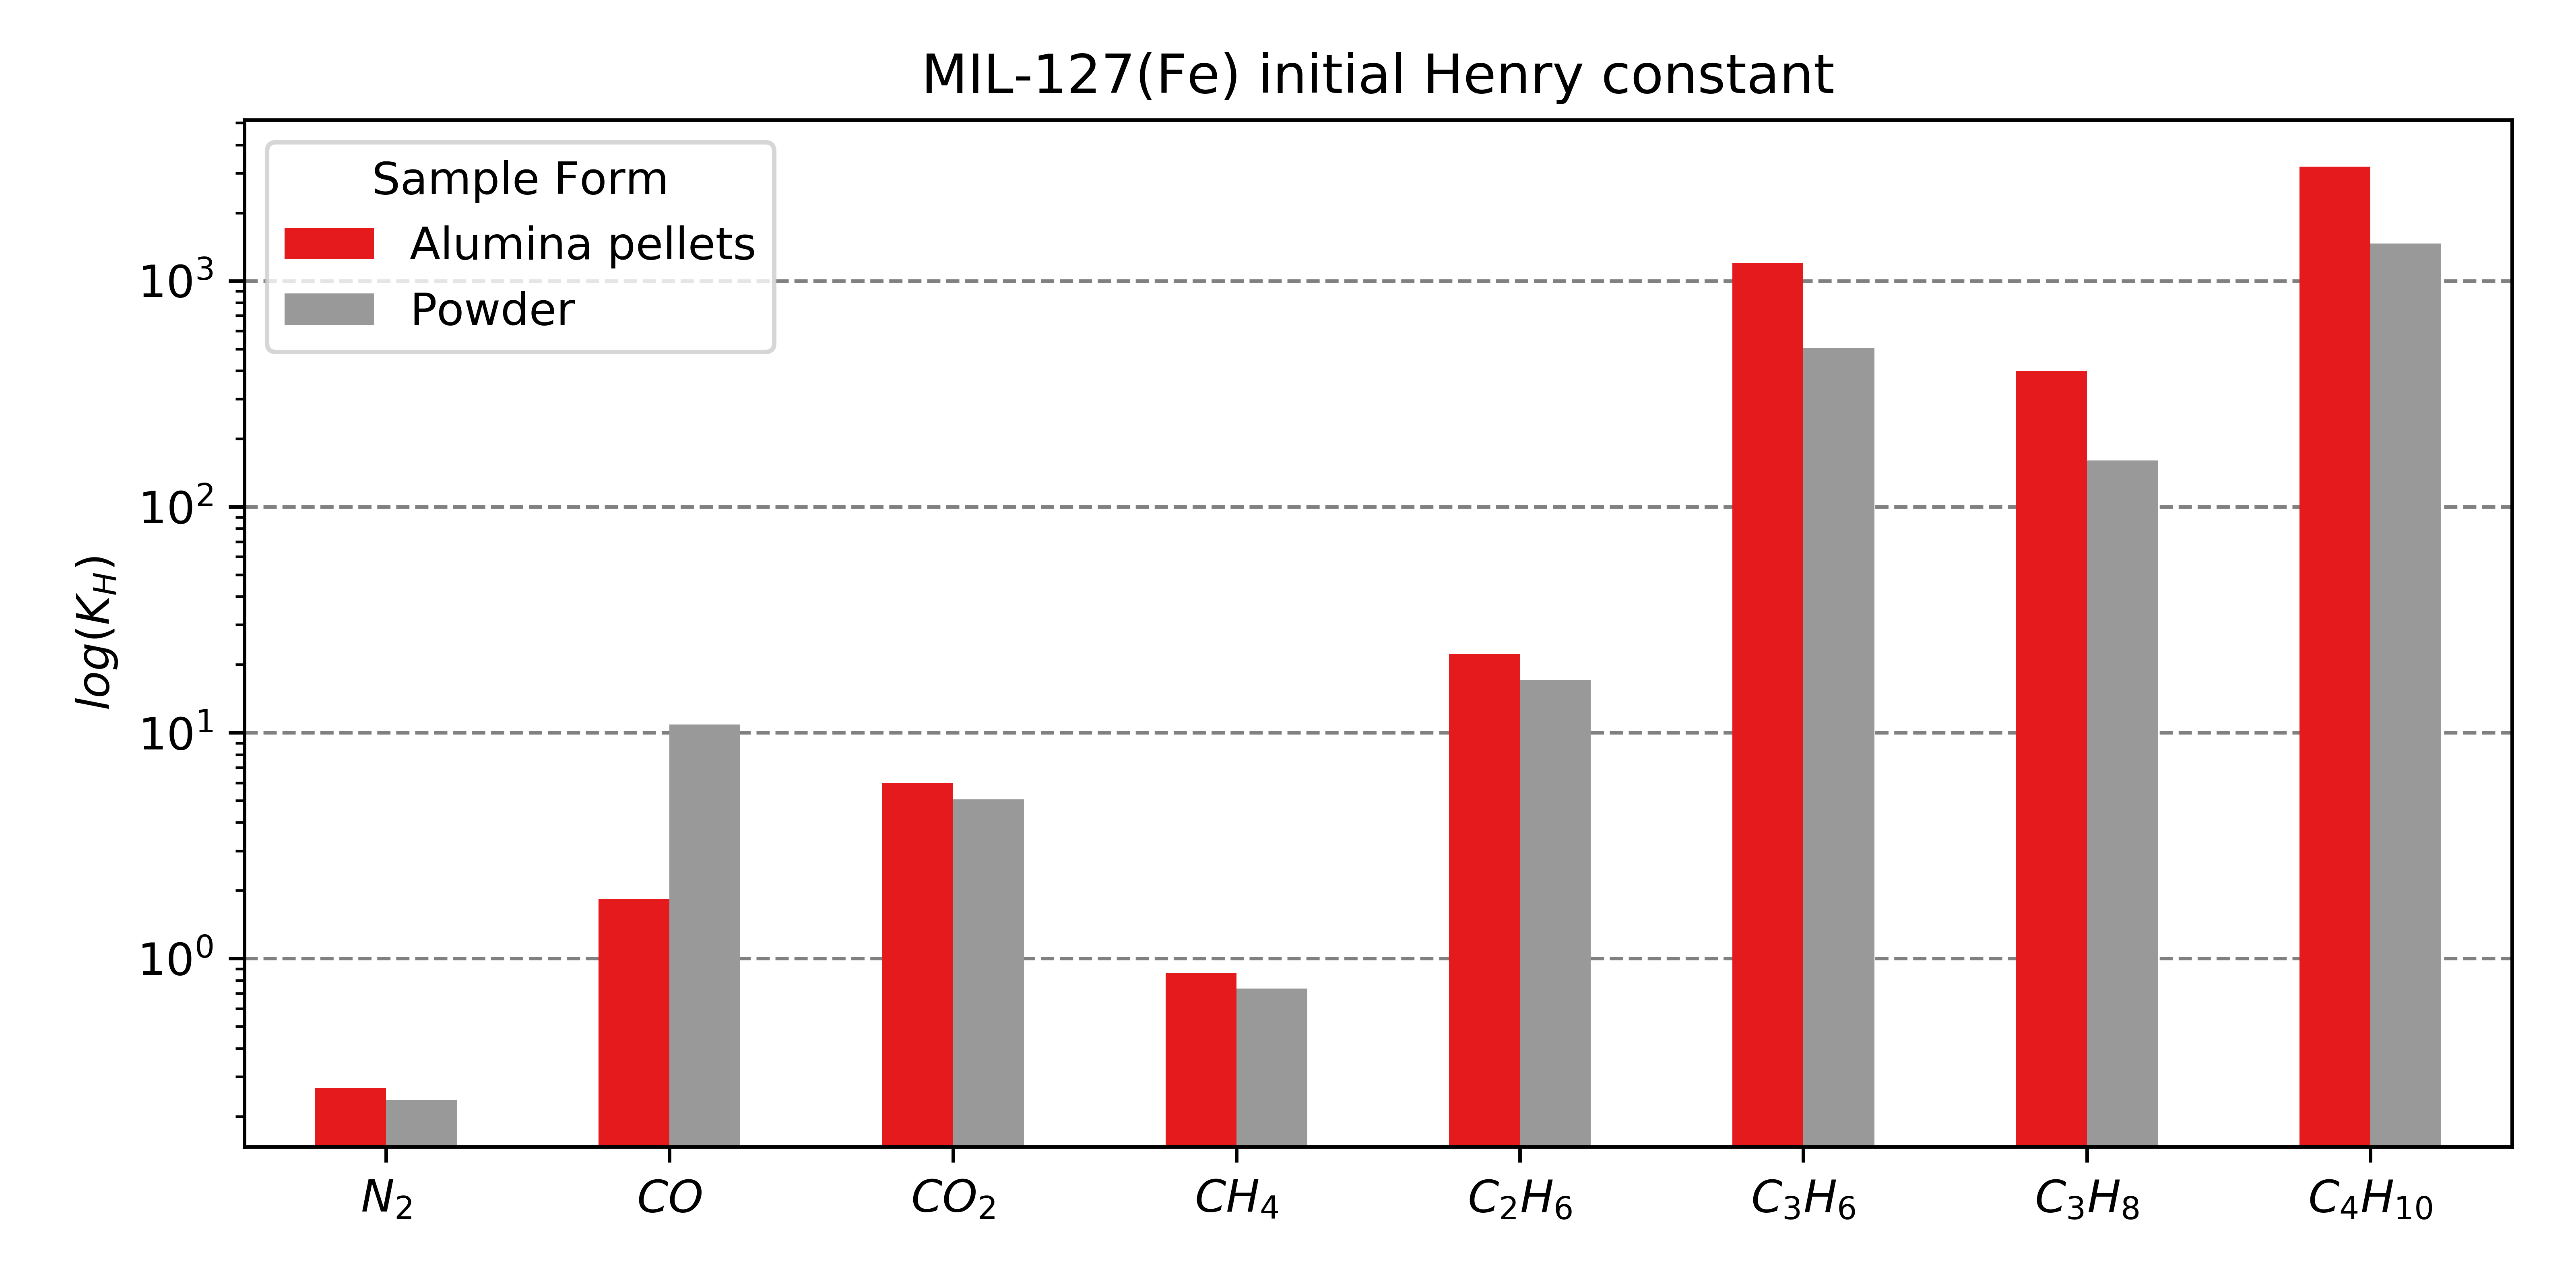
\includegraphics[width=\linewidth]{MIL-127(Fe)-henry-distribution}%
		}%
	\end{subfigure}%

	\begin{subfigure}{\linewidth}
		\parbox[c]{0.1\linewidth}{\caption{}%
			\label{shaping:fgr:analysismil127enth}}%
		\parbox[b]{0.8\linewidth}{%
			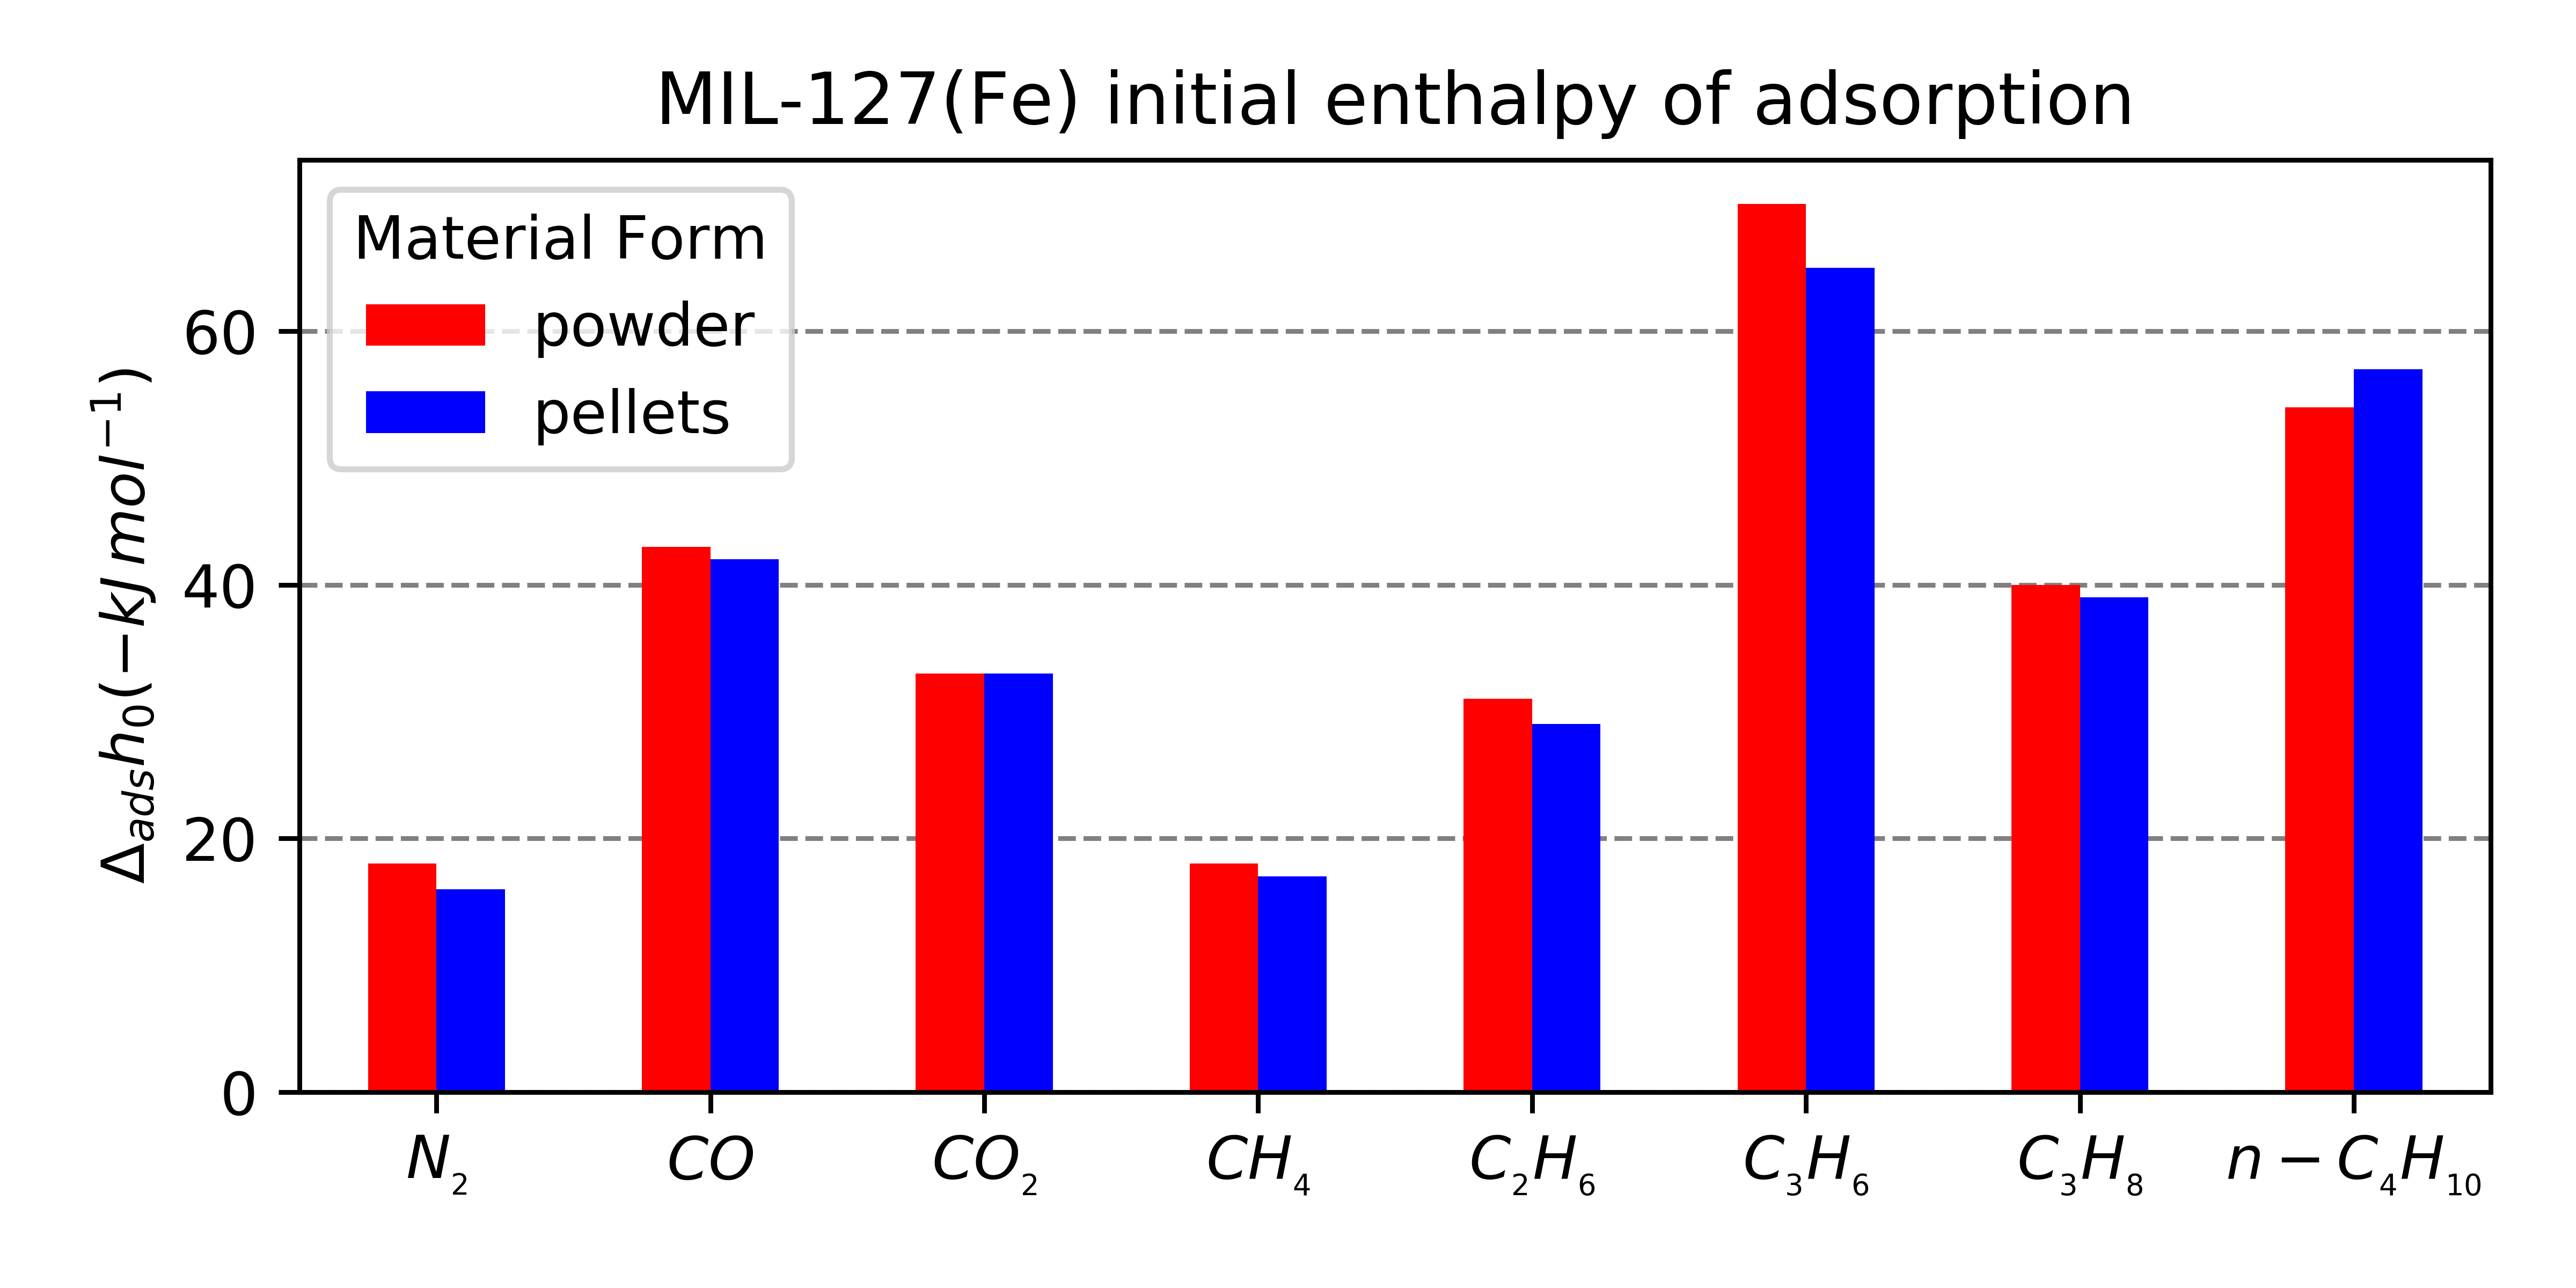
\includegraphics[width=\linewidth]{MIL-127(Fe)-enthalpy-distribution}%
		}%
	\end{subfigure}%

	\begin{subfigure}{\linewidth}
		\parbox[c]{0.1\linewidth}{\caption{}%
			\label{shaping:fgr:analysismil127basis}}%
		\parbox[b]{0.8\linewidth}{%
			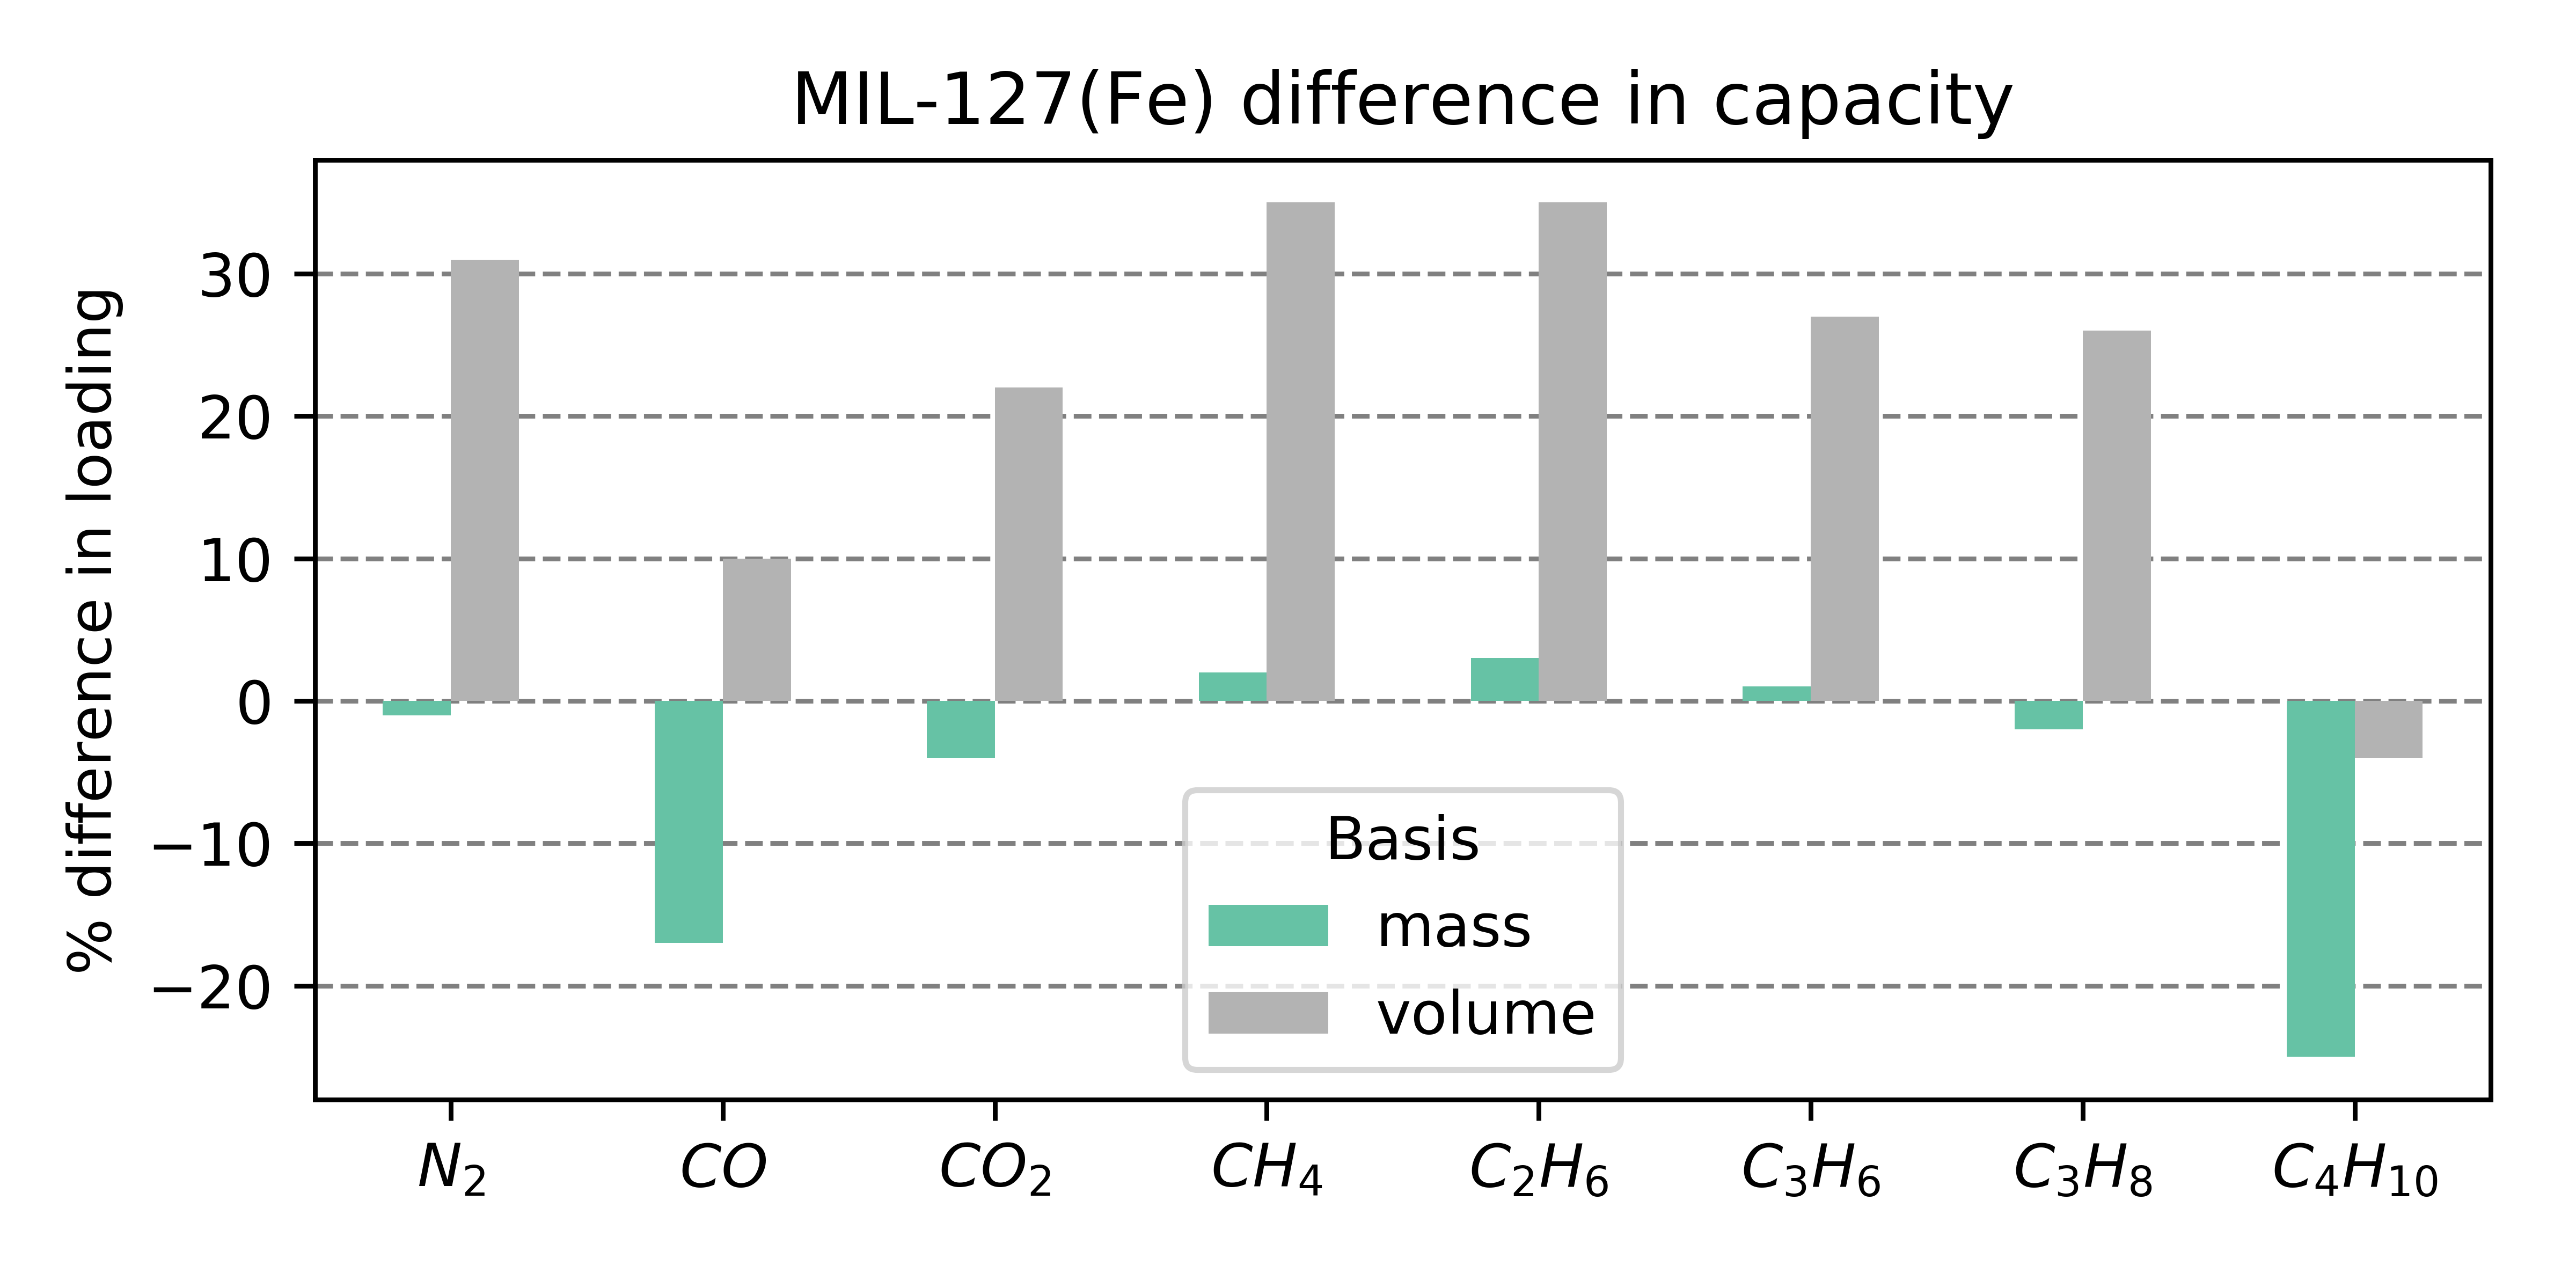
\includegraphics[width=\linewidth]{MIL-127(Fe)-mass-volume}%
		}%
	\end{subfigure}%

	\caption{KPIs extracted from the MIL-127(Fe) adsorption dataset with
		(a) logarithmic initial Henry constant (b) initial enthalpy of
        adsorption and (c) change in adsorption maximum capacity from 
        the powder to the alumina shaped version on a mass and volume 
        basis in red and grey respectively}%
	\label{shaping:fgr:analysismil127}
\end{figure}

\begin{figure}[!htb]
	\centering
	\begin{subfigure}{0.45\textwidth}
		\includegraphics[width=\linewidth]{calo/MIL-127(Fe)/c4h10-mass-basis-log-iso}
		\caption{\ce{C4H10} adsorption isotherms}%
		\label{shaping:fgr:mil127c4h10ads}
	\end{subfigure}%
	\begin{subfigure}{0.45\textwidth}
		\includegraphics[width=\linewidth]{calo/MIL-127(Fe)/co-enth}
		\caption{CO adsorption isotherms}%
		\label{shaping:fgr:mil127coads}
	\end{subfigure}%
	\caption{Selected isotherms from the MIL-127(Fe) dataset}%
	\label{shaping:fgr:mil127isotherms}
\end{figure}

The capacity comparison in \autoref{shaping:fgr:analysismil127basis}
paints an interesting picture. For most probes there is no change in
maximum loading showing that there is no structure degradation or
pore filling. Two outliers are apparent: carbon monoxide and
butane. The decrease in capacity on \ce{CO} can be explained through the
aforementioned changes in active site prevalence.
The drop in butane cannot be a consequence of the same effect
as there is a perfect overlap in the enthalpy curves as seen in
\autoref{shaping:fgr:mil127c4h10ads}.
Therefore it likely better explained through a size exclusion
effect as seen on UiO-66(Zr).

Overall, MIL-127(Fe) shows excellent performance when undergoing
alumina shaping, with almost no capacity loss, as long as
carbon monoxide or butane adsorption are required, where specific effects
come into play.
